\section{Histological Images Digitalization} \label{ssec:hist_im}
    Modern histopathology is essentially based on the careful interpretation of microscopic images, with the intention of correctly diagnose patients and to guide therapeutic decisions. In the last years, thanks to the quick development of scanning techniques and image processing, the discipline of histology have seen radical improvements: the main of which undoubtedly is the passage from the microscope's oculars to the computer's screen. This digitalization process has brought several advantages, that were previously impossible in classical histology, like telepathology and remote assistance in diagnosis processes, the integration with other digitalized clinical workflows, and patients' history, and most importantly the opening to applications of artificial intelligence.
    The name Whole Slide Imaging (WSI) refers to the modern virtual microscopy discipline, which consists of scanning a complete microscope slide and creating a single high-resolution digital file. This is commonly achieved by capturing many small high-resolution image tiles or strips and then montaging them to create a full image of a histological section. The four key steps of this process are image acquisition (scansion), editing, and on-screen image visualization.

    In the field of Digital Pathology (DP) an essential concept in image understanding is the magnification factor, which indicates the scale of representation of the image and allows dimension referencing. This factor is usually indicated as the magnification power of the microscope's lenses used during the analysis. After the digitalization process, this original magnification factor is prone to change, depending on the resolution of the visualization screen. Therefore, image resolution is measured in $\mu m$ per pixel, and it is set by the different composition of the acquisition chain, as the optical sensor and the lenses. Histological scanner are usually equipped with 20$\times$ or 40$\times$ objectives, which correspond to 0.5 and 0.25 $mm$/pixels resolution values. Lenses with 20$\times$ magnification factor are the most suitable for the great majority of histopathological evaluations, and it is the golden standard for scansions, for its good trade-off between image quality and time of acquisition. Scansions with 40$\times$ magnification could increase four-fold acquisition and processing time, final file's dimension, and storage cost. A single WSI image, acquired with 20$\times$ will occupy more than 600 MB alone.

    \begin{figure}
        \centering
        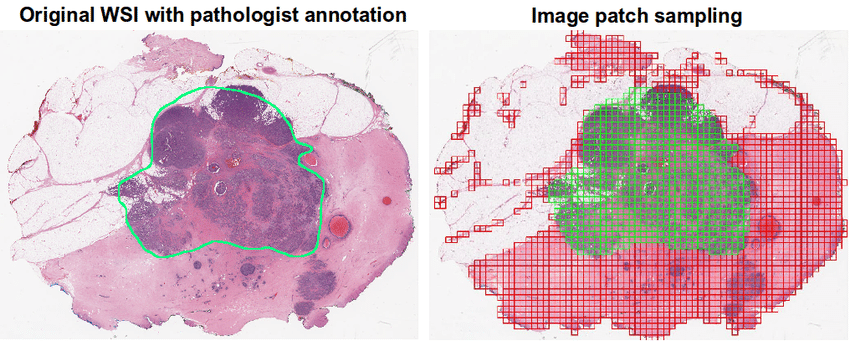
\includegraphics[width = \textwidth]{images/patches_grid}
        \caption{An example of whole slide image, with its grid decomposition in patches. It is visible the correspondence between a region of intereste maually anotated and the patches that matches that region. From \cite{WSI_grid}}
        \label{fig:patches_grid}
    \end{figure}

    Despite the WSI is a relatively mature discipline, it still struggles to integrate itself in the standard primitive diagnosis phase in histopathological laboratories. This is primarily due to some disadvantages, like images'resolution, image compression's artifacts, and auto-focusing algorithms, which plays a key role in the specimen interpretation. Furthermore, the scansion of histological samples is an additional step in the analysis which takes time. Despite the technological improvements the average time for the acquisition of a sample is around 5/10 minutes, depending on the number of slices in the slide, for just a single level of magnification. While in traditional histology, the pathologist has access to all the magnification levels at the same time. The real advantage, in fact, is in the long term. Once the images have been acquired they can be archived and consulted remotely almost instantaneously, helping clinical analysis and allowing remote assistance (telemedicine). Furthermore, the images now can be processed by artificial intelligence algorithms, allowing the application of technologies like Deep Learning which could revolutionize the research field, as already has been on many different disciplines in the scientific world.

    In order to allow to automatically process, such big images as the ones obtained through WSI, it is necessary to subdivide them in smaller patches. The dimension of which should be big enough to allow interpretation and to preserve a certain degree of representability of the original image. In Figure \ref{fig:patches_grid} is shown an example of a whole slide image, with its grid decomposition in patches. If the patches are too small, it should be over-specified for a particular region of tissue, loosing its general features. This could lead the learning algorithm to misinterpretation. However, this is not an exclusive limit of digital pathology, for a human pathologist would be impossible too to make solid decisions on a too limited sample of tissue. After the subdivision in patches, a typical process for biomedical images is the so-called \textit{data augmentation} of images, that is the process of creating re-newed images from the starting material through simple geometrical transformations, like translation, rotation, reflection, zoom in/out.

    The analysis of histological images usually consists of detecting the different components in the samples and to recognize their arrangement as a healthy or pathological pattern. It is necessary to recognize every sign of the vitality of the cells, evaluating the state of the nucleus. There are many additional indicators to consider the presence of inflammatory cells or tumoral cells. Furthermore, samples which are taken from different part of the human body present completely different characteristics, and this increase greatly the complexity of the analysis.
    A reliable examination of a sample thus requires a careful inspection made by a highly qualified expert. The automatization of this procedure would be extremely helpful, giving an incredible boost both in timing and accessibility. However, this is not a simple task and in section \ref{ssec:soa_seg} I will show some actual model for biomedical image processing in detail.

     \begin{figure}
         \centering
         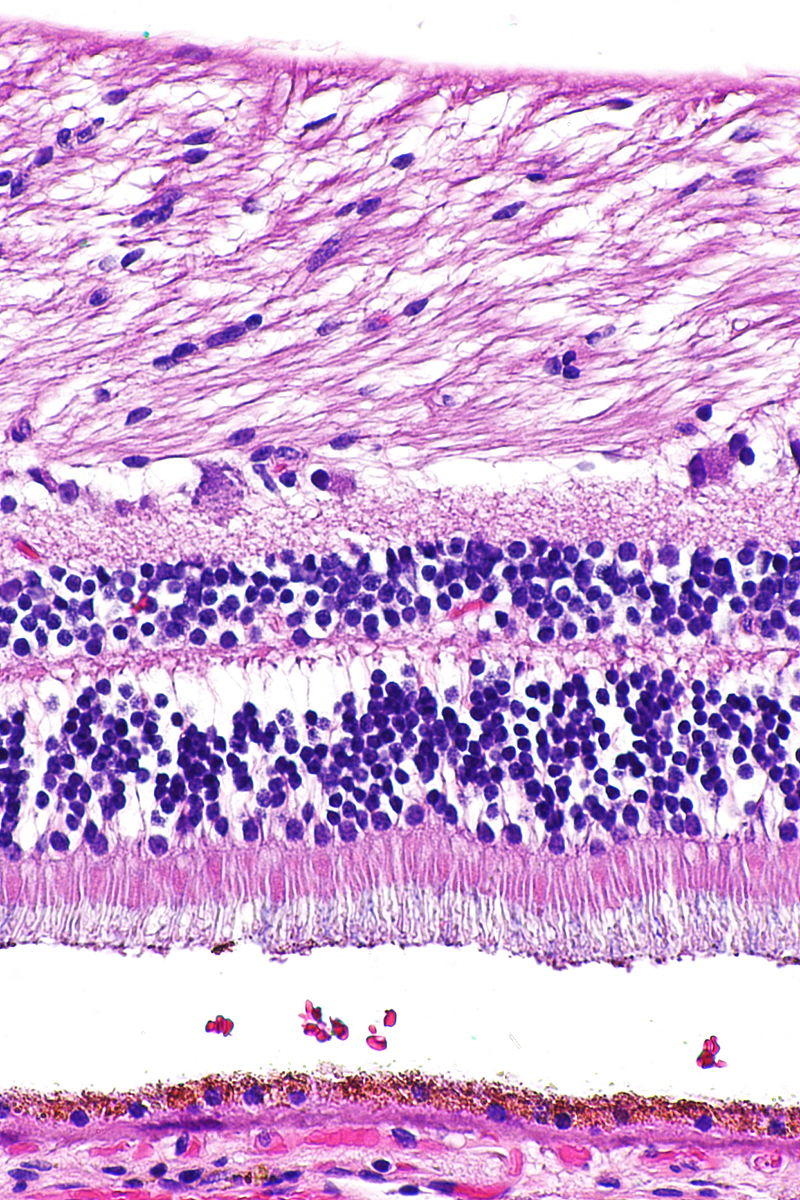
\includegraphics[width = 0.3\textwidth]{images/h&e_retyna}
         \caption{A sample of tissue from a retina (a part of the eye) stained with hematoxylin and eosin, cell nuclei stained blue-purple and extracellular material stained pink.}
         \label{fig:he_retyna}
     \end{figure}

\subsection{Slides Preparation for Optic Microscopic Observation} \label{ssec:samp_prep}
    In modern, as in traditional, histology regardless of the final support of the image the slide has to be physically prepared, starting from the sample of tissue. The sample and slide preparation is a crucial step for histological or cytological observation. It is essential to highlight what needs to be observed and to \textit{immobilize} the sample at a particular point in time and with characteristics close to those of its living state. There are five key steps for the preparation of samples \cite{Alturkistani2015}:
    \begin{description}
        \item [1) Fixation] is carried out immediately after the removal of the sample to be observed. It is used to immobilize and preserve the sample permanently in as life-like state as possible. It can be performed immersing the biological material in a formalin solution or by freezing, so immersing the sample in a tissue freezing medium which is then cooled in liquid nitrogen.

        \item [2) Embedding] if the sample has been stabilized in a fixative solution, this is the subsequent step. It consists in hardening the sample in a paraffin embedding medium, in order to be able to carry out the sectioning. It is necessary to dehydrate the sample beforehand, by replacing the water molecules in the sample with ethanol.

        \item [3) Sectioning] Sectioning is performed using microtomy or cryotomy. Sectioning is an important step for the preparation of slides as it ensures a proper observation of the sample by microscopy. Paraffin-embedded samples are cut by cross-section, using a microtome, into thin slices of 5 $\mu m$. Frozen samples are cut using a cryostat. The frozen sections are then placed on a glass slide for storage at -80$\degree$C. The choice of these preparation conditions is crucial in order to minimize the artifacts. Paraffin embedding is favored for preserving tissues; freezing is more suitable for preserving DNA and RNA and for the labeling of water-soluble elements or of those sensitive to the fixation medium.

        \item [4) Staining] Staining increases contrasts in order to recognize and differentiate the different components of the biological material. The sample is first deparaffinized and rehydrated so that polar dyes can impregnate the tissues. The different dyes can thus interact with the components to be stained according to their affinities. Once staining is completed, the slide is rinsed and dehydrated for the mounting step.

    \end{description}

    Hematoxylin and eosin stain (H\&E) is one of the principal tissue stains used in histology \cite{he_stain}, and it is the most widely used stain in medical diagnosis and is often the gold standard \cite{Rosai2007}. H\&E is the combination of two histological stains: hematoxylin and eosin. The hematoxylin stains cell nuclei blue, and eosin stains the extracellular matrix and cytoplasm pink, with other structures taking on different shades, hues, and combinations of these colors. An example of H\&E stained is shown in Figure \ref{fig:he_retyna}, in which we can see the typical color palette of a histological specimen.

\subsection{Pancreas Microanatomy and Tumoral Evidences} \label{ssec:pancr_anat}
    The Pancreas is an internal organ of the human body, part of both the digestive system and the endocrine system. It acts as a gland with both endocrine and exocrine functions, and it is located in the abdomen behind the stomach. Its main endocrine duty is the secretion of hormones like insulin and glucagon which are responsible for the regulation of sugar levels in the blood. As a part of the digestive system instead, it acts as an exocrine gland secreting pancreatic juice, which has an essential role in the digestion of many different nutritional compounds. The majority of pancreatic tissue has a digestive role, and the cells with this role form clusters called \textit{acini} around the small pancreatic ducts. The acinus secrete inactive digestive enzymes called zymogens into the small intercalated ducts which they surround, and then in the pancreatic blood vessels system \cite{Pancreas}. In Figure \ref{fig:panc_struct} is shown a picture of the pancreas, with its structure and its placement in the human body. All the tissue is actually rich in other important elements as the islets of Langerhans that have an important role in the endocrine action of the pancreas. All over the structure is present a layer of connective tissue which are clearly visible in the traditional histological specimens.

     \begin{figure}
         \centering
         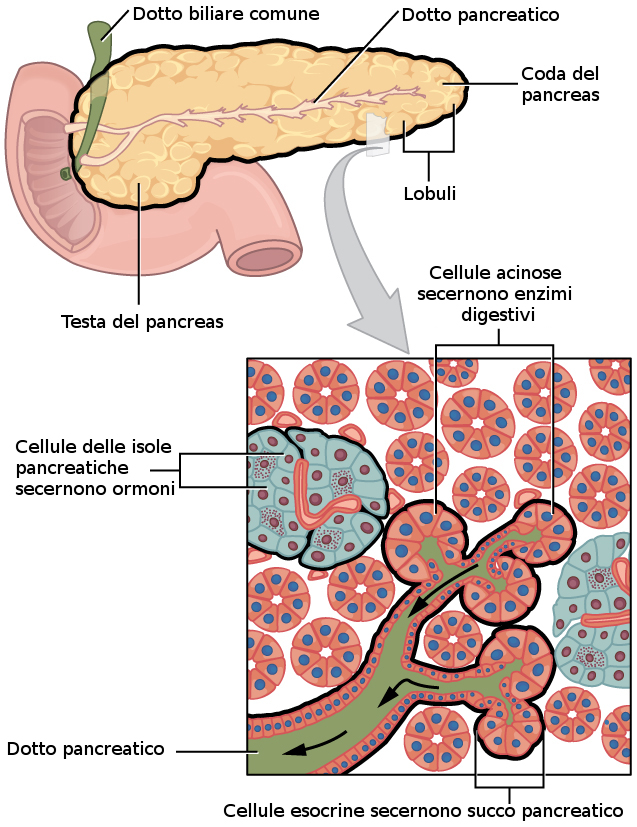
\includegraphics[width = 0.45\textwidth]{images/pancr_struct_zoom}
         %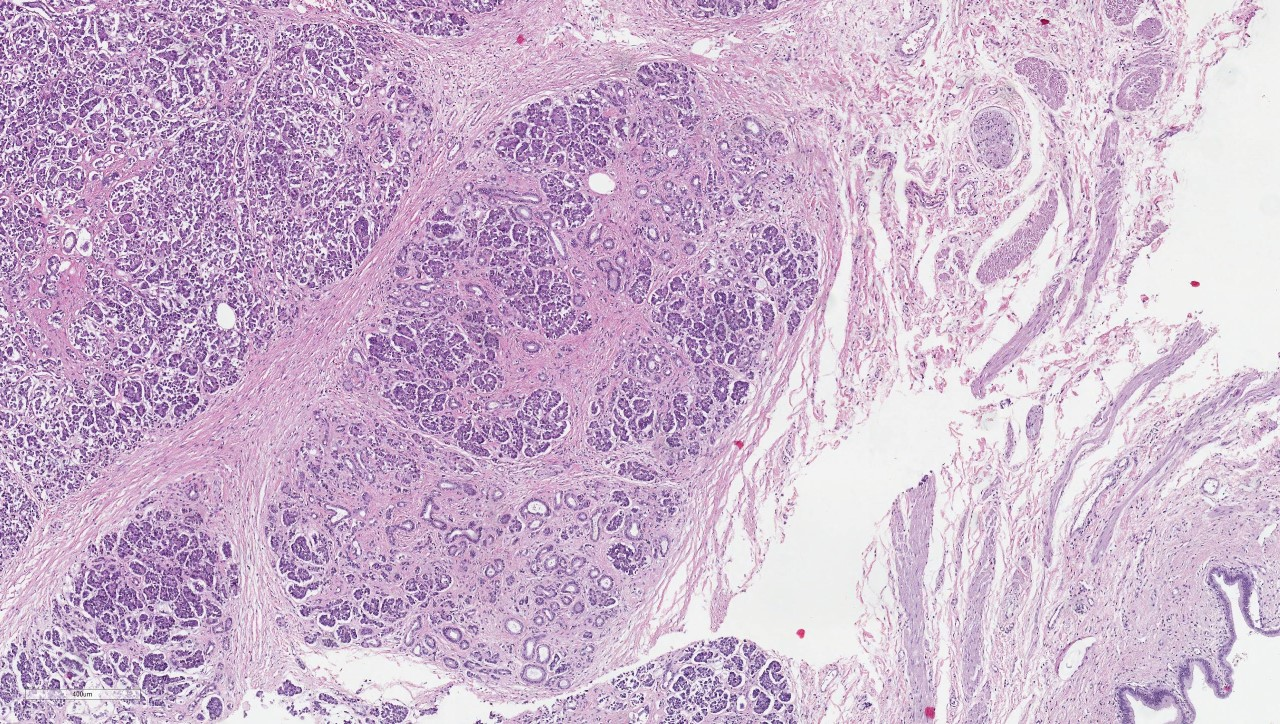
\includegraphics[width = 0.45\textwidth]{images/panc_specimen}
         \caption{A picture of pancreas' structure in its physiological context. In this picture is clearly visible the macroscopic structure and the glandular organization at microscopic level.}
         \label{fig:panc_struct}
     \end{figure}

    There are many tumoral diseases interest the pancreas, they represent one of the main causes of decease for cancer in occidental countries, and its incidence rate in Europe and the USA has risen significantly in the last decades. There are two main kinds of pancreatic neoplasms: endocrine and exocrine pancreatic tumors. The endocrine pancreas neoplasms derive from the cells constituting the Langherans' islets and are typically divided into functioning and non-functioning ones, depending on the capability of the organs to secrete hormones. Those diseases might be benign or malignant and they can have a different degree of aggressivity. Exocrine pancreatic tumors tough are the most frequent ones. Among those, the great majority of episodes are of malignant neoplasms, and in particular, the ductal adenocarcinoma is the most frequent form of disease, responsible alone for the 95\% of the cases. From a macroscopic point of view, those tumors are characterized by an abundant fibrotic stroma\footnote{Stroma is the part of a tissue or organ with a structural or connective role. It is made up of all the parts without specific functions of the organ like connective tissue, blood vessels, ducts, etc. The other part, the parenchyma, consists of the cells that perform the function of the tissue or organ.}, which can represent over 50\% of the tumor's mass and it is responsible for the hard-ligneous tumor's aspect. This disease is frequently followed by pancreatitis episodes.

    From a microscopical point of view, this tumor is characterized by the presence of glandular structures, made by one or more layers of columnar or cuboidal epithelial cells embedded in fibrotic parenchyma. The histological inspection of a sample of pancreatic tissue allows us to grade the stadium of the disease. While analyzing a specimen the operator looks for some specific markers like the glandular differentiation in tubular and ductal structure, the degree of production of mucin, the percentage of cells in the mitotic phase, and the degree of tissue nuclear atypia. The evaluation of those characters allows us to assign a degree of development form I to III to the specific case of ductal adenocarcinoma.

    During the microscopical analysis of a histological sample, there are other interesting markers to be evaluated, as a specific set of lesions which goes under the name of PanIN (Pancreatic Intraepithelial Neoplasia) and could not be appreciated with other diagnostic techniques. PanIN describes a wide variety of morphological modifications, differentiated on the degree of cytological atypia and architectural alterations \cite{pmid18787611}. A careful analysis of a histological sample of tissue after a biopsy is a fundamental step in the treatment of a patient.

\subsection{Skin Microanatomy and Tumoral Evidences} \label{ssec:derm_anat}
    Skin is the layer of soft, flexible outer tissue covering the body of a vertebrate animal, with the three main functions of protection, regulation, and sensation. Mammalian skin is composed of two primary layers: the epidermis, which provides waterproofing and serves as a barrier to infection, and the dermis, which serves as a location for the appendages of skin. The epidermis is composed of the outermost layers of the skin. It forms a protective barrier over the body's surface, responsible for keeping water in the body and preventing pathogens from entering, and is a stratified squamous epithelium, composed of proliferating basal and differentiated suprabasal keratinocytes. The dermis is the layer of skin beneath the epidermis that consists of connective tissue and cushions the body from stress and strain. The dermis provides tensile strength and elasticity to the skin through an extracellular matrix composed of collagen fibrils, microfibrils, and elastic fibers, embedded in hyaluronan and proteoglycans.

    \begin{figure}
        \centering
        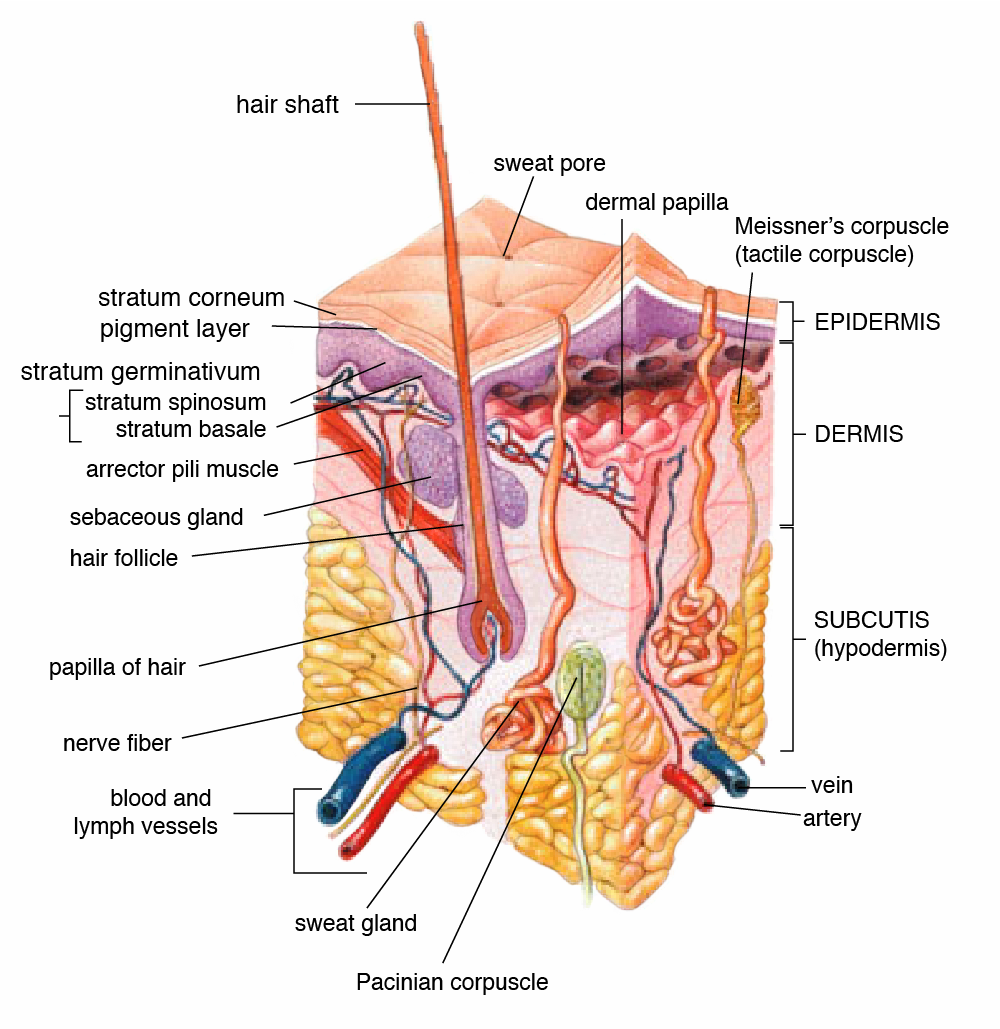
\includegraphics[width = 0.45\textwidth]{images/derm_scheme}
        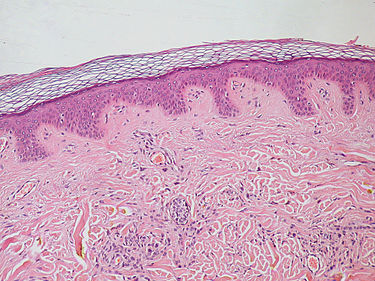
\includegraphics[width = 0.45\textwidth]{images/derm_specimen}

        % \begin{subfigure}[b]{0.45\textwidth}
        %      \centering
        %      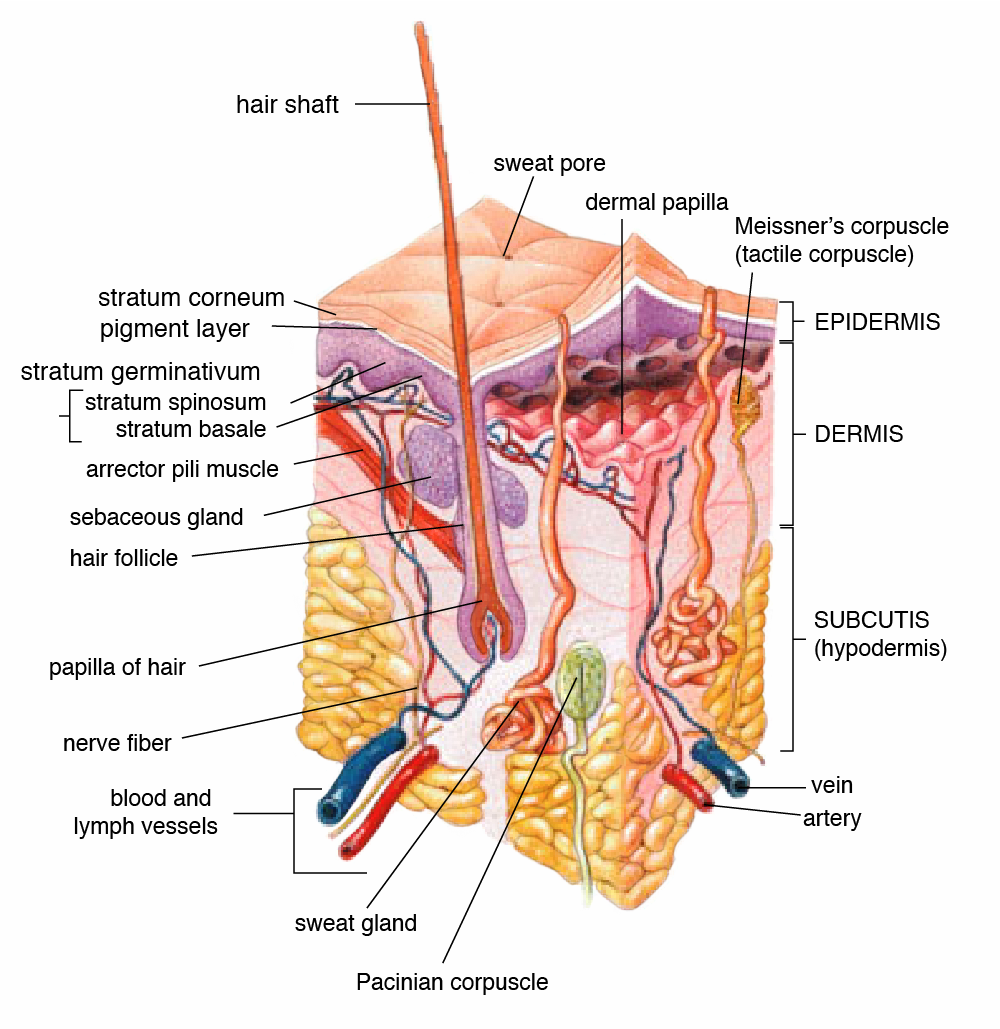
\includegraphics[width = \textwidth]{images/derm_scheme}
        %      \caption{}
        %      \label{fig:derm_scheme}
        % \end{subfigure}
        % \hfill
        % \begin{subfigure}[b]{0.45\textwidth}
        %      \centering
        %      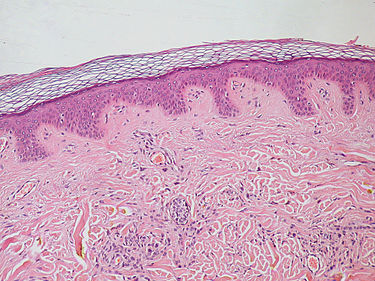
\includegraphics[width = \textwidth]{images/derm_specimen}
        %      \caption{}
        %      \label{fig:derm_specimen}
        % \end{subfigure}
        \caption{(left) Microanatomical description of a region of dermal tissue and all the interesting elements present in cutis, and subcutaneous layer. (right) An actual histological specimen from a sample of dermal tissue.}
        \label{fig:derm_descr}
    \end{figure}

    Melanoma is the most aggressive form of skin tumor. It is the second most frequent tumors in men under 50 years, and the third for women under 50 years, with over than 12.300 cases in Italy every year. Melanoma is considered nowadays a multifactorial pathology, which originates from the interaction between genetic susceptibility and environmental exposure. The most important environmental risk factor is the intermittent solar exposure, for the genotoxic effect of ultraviolet rays on the skin. Different studies show also a strong correlation between the total number of nevi on the skin and the incidence of melanoma.


% nevi atipici sono lesioni melanocitarie acquisite benigne che condividono alcune caratteristiche del melanoma, quali l’asimmetria, i bordi irregolari, la colorazione disomogenea, il diametro maggiore di 5 mm. Talvolta gli aspetti istopatologici di alcuni nevi clinicamente atipici possono essere del tutto tranquillizzanti, ma a livello epidemiologico un numero elevato di nevi atipici può correlare con un aumentato rischio di melanoma; una metanalisi di studi osservazionali, infatti, ha evidenziato che il rischio relativo di sviluppare un melanoma è di 1.5 nei soggetti con un nevo atipico e di 6.36 nei soggetti con 5 o più.8

    We can distinguish two separated phases in the growth of melanoma: the radial phase, in which the proliferation of malignant melanocytes is limited to the epidermis, and the vertical phase, where malignant melanocytes form nests or nodules in the dermis. The dermatological analysis should distinguish which specific type of melanoma is affecting the patient. There are many types of melanoma:
    \begin{description}
        \item [Superficial Spreading Melanoma]: This is the most common subtype, and it represents alone more than the 75\% of all melanoma cases. These neoplasms show relatively large malignant melanocytes, inflammatory cells (epithelioid), and an abundance of cytoplasm.

        \item [Lentigo Maligna Melanoma]: It typically arises in photodamaged skin regions. Neplasmatic melanocytes are of polygonal shape, with hyperchromatic nuclei, and they are followed by a reduction in the cytoplasm.

        \item [Acral lentiginous melanoma]: It typically arises on palmar, plantar, subungual, or mucosal surfaces. Melanocytes are usually arranged along the dermal-epidermal junction. The progression of this type of melanoma is characterized by the presence of large junctional nests of atypical melanocytes, which are extended and hyperchromatic, with a shortage of cytoplasm.

        \item [Modular Melanoma]: By definition, this is the melanoma with a pure vertical growth. It is followed by the presence of numerous little tumoral nests of neoplastic melanocytes, with a high rate of mitotic state, arranged to form a single big nodule.
    \end{description}

    The careful examination of histological samples extracted from the tissue under analysis is the most important step for the assessment of the actual form of neoplasms.
